\documentclass{article}
\usepackage{xcolor}
\newcommand{\red}{\color{red}}
\usepackage{tikz}
\usepackage[width=128mm]{geometry}
\pagestyle{empty}

\begin{document}

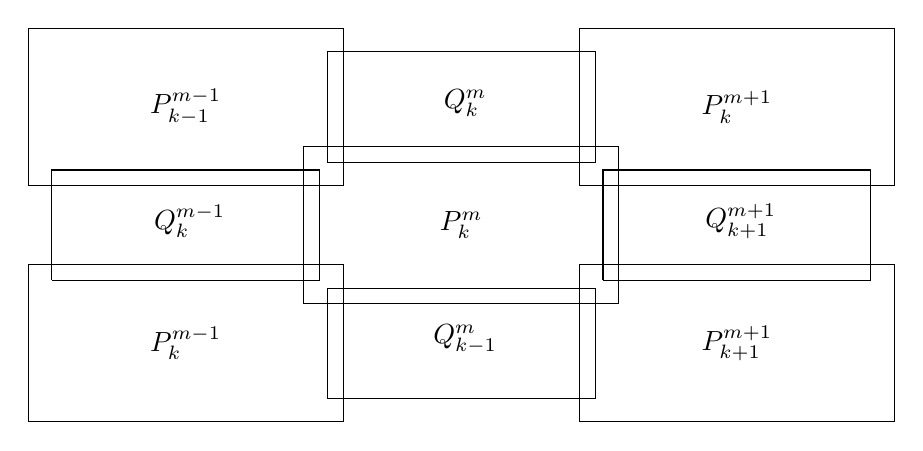
\begin{tikzpicture}
	\draw
	%% P
	(0,0) -- +(4,0) -- +(4,2) -- +(0,2) -- +(0,0) +(2,1) node{$P_{k}^{m-1}$}
	(0,3) -- +(4,0) -- +(4,2) -- +(0,2) -- +(0,0) +(2,1) node{$P_{k-1}^{m-1}$}
	(3.5,1.5) -- +(4,0) -- +(4,2) -- +(0,2) -- +(0,0) +(2,1) node{$P_{k}^{m}$}
	(7,0) -- +(4,0) -- +(4,2) -- +(0,2) -- +(0,0) +(2,1) node{$P_{k+1}^{m+1}$}
	(7,3) -- +(4,0) -- +(4,2) -- +(0,2) -- +(0,0) +(2,1) node{$P_{k}^{m+1}$}
	%% Q
	(.3,1.8) -- ++(0,1.4) -- ++(3.4,0) -- ++(0,-1.4) -- ++(-3.4,0) +(1.75,0.75) node{$Q_{k}^{m-1}$}
	(3.8,0.3) -- ++(0,1.4) -- ++(3.4,0) -- ++(0,-1.4) -- ++(-3.4,0) +(1.75,0.75) node{$Q_{k-1}^{m}$}
	(3.8,3.3) -- ++(0,1.4) -- ++(3.4,0) -- ++(0,-1.4) -- ++(-3.4,0) +(1.75,0.75) node{$Q_{k}^{m}$}
	(7.3,1.8) -- ++(0,1.4) -- ++(3.4,0) -- ++(0,-1.4) -- ++(-3.4,0) +(1.75,0.75) node{$Q_{k+1}^{m+1}$}
	;
\end{tikzpicture}

\end{document}
